% ---------------------------------------------------------------------------- %

\section{Especificação da Camada de Negócio}
\label{cap:negocio}

A camada de negócio engloba toda a lógica interna do sistema e as suas responsabilidades passam pelo processamento dos pedidos provenientes da camada de apresentação por forma a cumprir os requisitos funcionais do sistema, bem como assegurar o cumprimento de requisitos não-funcionais.

Assim para especificar a mesma recorreu-se a um diagrama de classes que irá apresentar as diversas classes que constituem esta camada, bem como abordar de forma mais especifica todas as componentes das mesmas e diagramas de sequência que demonstram e descrevem a interação entre essas classes.

Um diagrama de pacotes onde se pode ver a estrutura genérica da camada de negócio foi já fornecido no \refcap{cap:arquitetura}, apresentado na \reffig{fig:arquitetura:DiagramaPacotes}, sendo o pacote referente à camada de negócio o \emph{Model}.

\subsection{Diagramas de classes}
\label{subsec:diagramas_classe}

O presente diagrama de classes apresenta então como classes constituintes da camada de negócio, as classes:

\begin{itemize}
    \item Bela Sopa;
    \item Utilizador;
    \item Administrador;
    \item Cliente;
    \item Localização;
    \item Ementa Semanal;
    \item Loja;
    \item Receita;
    \item Processo;
    \item Tarefa;
    \item Ingrediente;
    \item Utensílios;
    \item Técnicas.
\end{itemize}

As relações entre as entidade são também descritas no diagrama, fornecendo uma vista geral da estrutura do sistema.

 \begin{figure}[H]
   \centering
   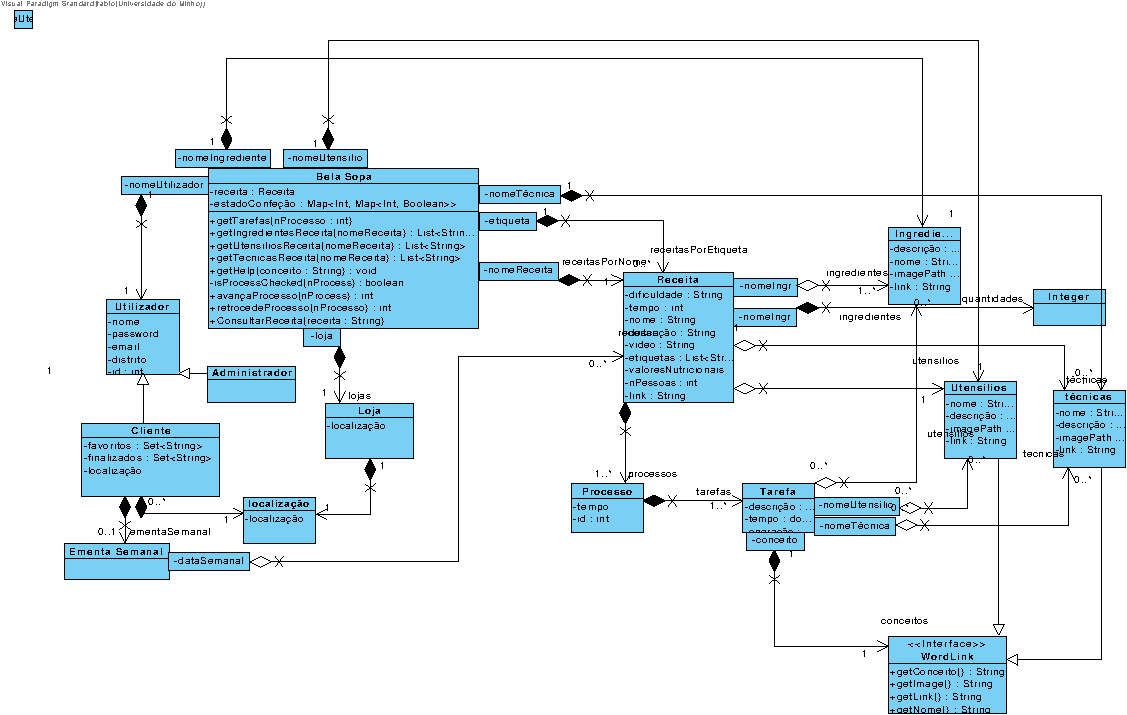
\includegraphics[width=\textwidth]{figures/10/Diagrama_Classes.pdf}
   \caption{Diagrama de classes para a camada de negócio.}
   \label{fig:negocio:DiagramaClasses}
 \end{figure}

\subsection{Diagramas de sequência}
\label{subsec:diagramas_sequencia}

Para demonstrar as classes que compõem a camada de negócio, a forma como estas se relacionam e interatuam entre si, e as suas funções, apresentam-se, a título ilustrativo, os diagramas de sequência de dois eventos do sistema:

\begin{itemize}
    \item Confecionar Receita;
    \item Consultar Receita.
\end{itemize}

\begin{figure}[H]
   \centering
   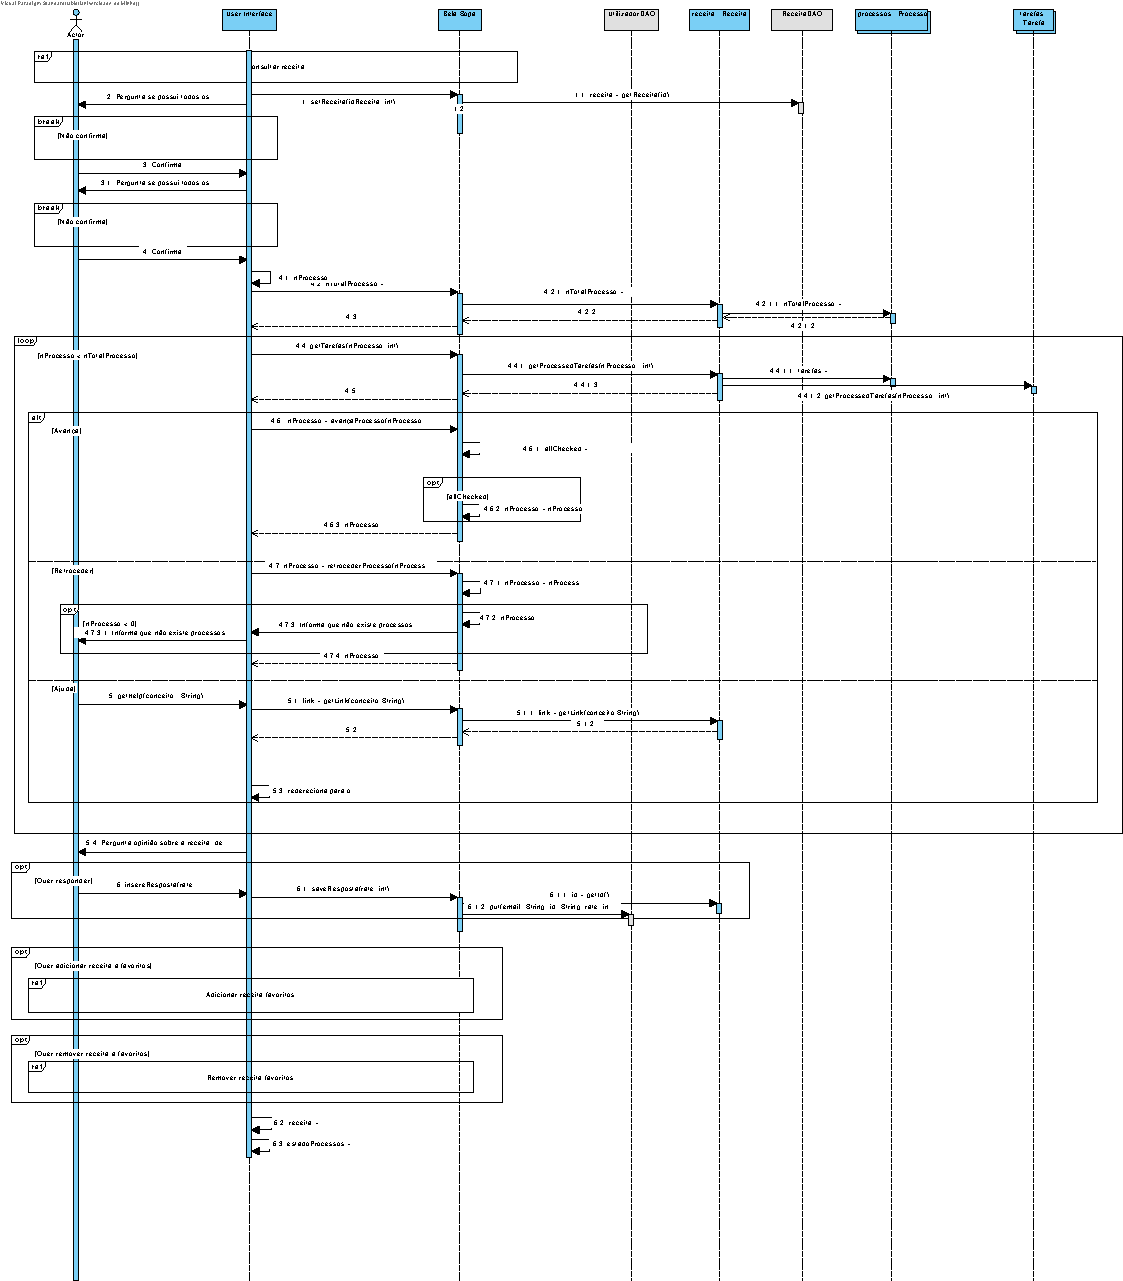
\includegraphics[width=\textwidth]{figures/10/Confecionar_receita.pdf}
   \caption{Diagrama de sequência para a confeção de uma receita.}
   \label{fig:negocio:DiagramaSequencia1}
 \end{figure}

\begin{figure}[H]
   \centering
   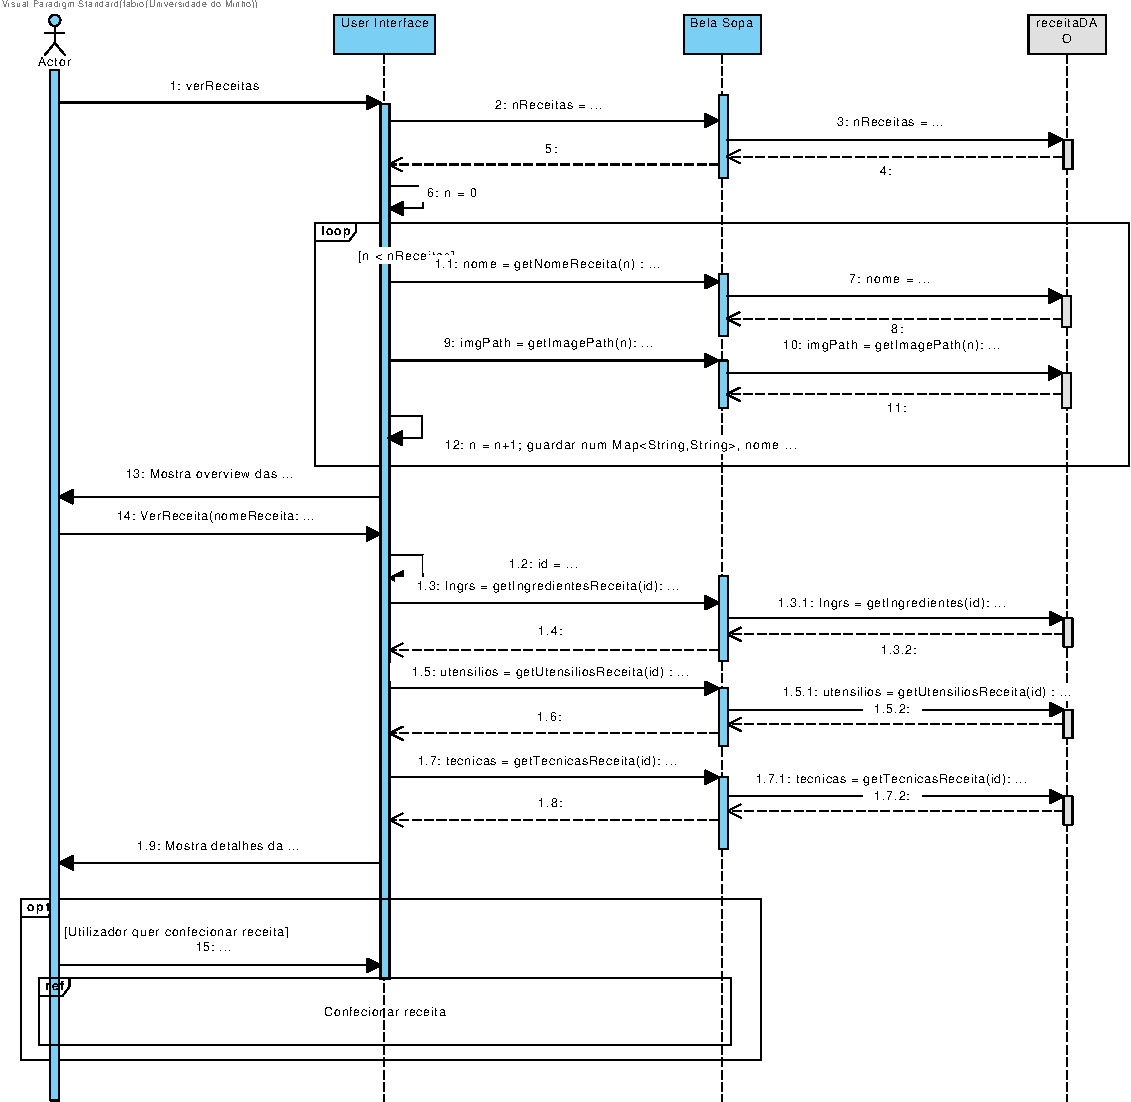
\includegraphics[width=\textwidth]{figures/10/Consultar_receita.pdf}
   \caption{Diagrama de sequência para a consulta de uma receita.}
   \label{fig:negocio:DiagramaSequencia2}
 \end{figure}
 
 Os restantes diagramas de sequência podem ser encontrados no \refane{ane:negocio-diag-seq}. 

% ---------------------------------------------------------------------------- %
